\documentclass[compress]{beamer}
\usepackage{ifthen,verbatim}

\newcommand{\isnote}{}
\xdefinecolor{lightyellow}{rgb}{1.,1.,0.25}
\xdefinecolor{darkblue}{rgb}{0.1,0.1,0.7}

%% Uncomment this to get annotations
%% \def\notes{\addtocounter{page}{-1}
%%            \renewcommand{\isnote}{*}
%% 	   \beamertemplateshadingbackground{lightyellow}{white}
%%            \begin{frame}
%%            \frametitle{Notes for the previous page (page \insertpagenumber)}
%%            \itemize}
%% \def\endnotes{\enditemize
%% 	      \end{frame}
%%               \beamertemplateshadingbackground{white}{white}
%%               \renewcommand{\isnote}{}}

%% Uncomment this to not get annotations
\def\notes{\comment}
\def\endnotes{\endcomment}

\setbeamertemplate{navigation symbols}{}
\setbeamertemplate{headline}{\mbox{ } \hfill
\begin{minipage}{5.5 cm}
\vspace{-0.75 cm} \small
\end{minipage} \hfill
\begin{minipage}{4.5 cm}
\vspace{-0.75 cm} \small
\begin{flushright}
\ifthenelse{\equal{\insertpagenumber}{1}}{}{Jim Pivarski \hspace{0.2 cm} \insertpagenumber\isnote/\pageref{numpages}}
\end{flushright}
\end{minipage}\mbox{\hspace{0.2 cm}}\includegraphics[height=1 cm]{../cmslogo} \hspace{0.1 cm} \includegraphics[height=1 cm]{../tamulogo} \hspace{0.01 cm} \vspace{-1.05 cm}}

\begin{document}
\begin{frame}
\vfill
\begin{center}
\textcolor{darkblue}{\Large Track-based Alignment of the Muon System}

\vfill
\begin{columns}
\column{0.3\linewidth}
\begin{center}
\large
\textcolor{darkblue}{Jim Pivarski}

\vspace{0.2 cm}
Alexei Safonov
\end{center}

\column{0.3\linewidth}
\begin{center}
\large
K\'aroly Banicz
\end{center}

\column{0.3\linewidth}
\begin{center}
\large
Pablo Martinez Ruiz del Arbol

\vspace{0.2 cm}
\ldots
\end{center}
\end{columns}

\begin{columns}
\column{0.3\linewidth}
\begin{center}
\scriptsize
{\it Texas A\&M University}
\end{center}
\column{0.3\linewidth}
\begin{center}
\scriptsize
{\it US-CMS}
\end{center}
\column{0.3\linewidth}
\begin{center}
\scriptsize
{\it IFCA}
\end{center}
\end{columns}

\vfill
23 September, 2008

\end{center}
\end{frame}

%% \begin{notes}
%% \item This is the annotated version of my talk.
%% \item If you want the version that I am presenting, download the one
%% labeled ``slides'' on Indico (or just ignore these yellow pages).
%% \item The annotated version is provided for extra detail and a written
%% record of comments that I intend to make orally.
%% \item Yellow notes refer to the content on the {\it previous} page.
%% \item All other slides are identical for the two versions.
%% \end{notes}

\begin{frame}
\frametitle{Outline}
\begin{itemize}\setlength{\itemsep}{0.75 cm}
\item 
\end{itemize}
%% \hspace{-0.83 cm} \textcolor{darkblue}{\Large Outline2}
\end{frame}

%% \section*{First section}
%% \begin{frame}
%% \begin{center}
%% \Huge \textcolor{blue}{First section}
%% \end{center}
%% \end{frame}

\begin{frame}
\frametitle{CSC alignment parameters}

\begin{columns}
\column{0.35\linewidth}
\small

\begin{itemize}\setlength{\itemsep}{0.1 cm}
\item Align two parameters: $r\phi$ positions around beamline
with $\varphi_y$ angles around chamber center as a pre-requisite
\item 10~mrad $\varphi_y$ error $\to$ 1.25~mm $r\phi$ mistake
\item Align two rings: ME$-$2/1 ME$-$3/1, to make use of overlaps tracks and straight-through tracks
\item Run 62232: \mbox{2/3 of full \hspace{-0.5 cm}} statistics \mbox{in short time\hspace{-1 cm}}
\end{itemize}

\column{0.65\linewidth}

\includegraphics[width=0.38\linewidth]{one_chamber.png} 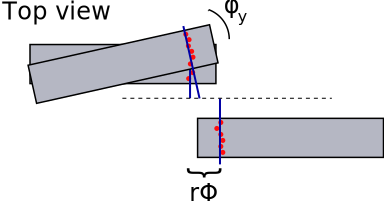
\includegraphics[width=0.62\linewidth]{order_of_parameters.png}

\vspace{1 cm}

\includegraphics[width=\linewidth]{overlaps_straight_through.png}

\end{columns}
\end{frame}

\begin{frame}
\frametitle{Determining $\varphi_y$}
\small

\begin{columns}
\column{0.6\linewidth}

\begin{itemize}
\item Two independent methods:
\begin{itemize}
\item $d\phi/dz$ slope must agree in both chambers of an overlap track, calculate solution of 18 relative corrections
\item $d\phi/dz$ slope must be on average zero, because beam-halo tracks come from the LHC
\end{itemize}
\item \mbox{Disjoint sets of tracks, same pattern of results, well under 10~mrad\hspace{-5 cm}}
\end{itemize}

\column{0.4\linewidth}
\includegraphics[width=\linewidth]{track_lhc_plane_closeup.png}
\end{columns}

\vspace{-0.2 cm}
\begin{columns}
\column{0.2\linewidth}
\begin{center}
\only<1>{before correction:}\only<2>{after correction:

\vspace{0.1 cm}
\scriptsize{(from LHC pointing)}}
\end{center}
\column{0.65\linewidth}
\begin{center}
\only<1>{\includegraphics[height=\linewidth, angle=90]{angle_comparison_meminus21.pdf}}
\only<2>{\includegraphics[height=\linewidth, angle=90]{angle_seconditer_meminus21.pdf}}
\end{center}
\end{columns}
\end{frame}

\begin{frame}
\frametitle{Another cross-check for $\varphi_y$}
\small

$d\phi/dz$ of ME$-$2/1 segment must match $d\phi/dz$ of ME$-$3/1 segment

Quality of $-$2/1 to $-$3/1 angular match before and after correction:
\begin{center}
\includegraphics[height=0.65\linewidth, angle=90]{angle_matching.pdf} chambers 13--16 have too few tracks for precision
\end{center}

To summarize,
\begin{enumerate}
\item Observed solution of relative $\varphi_y$ corrections around the ring (overlaps tracks in each station separately: $N$ vs.\ $N+1$)
\item Applied absolute $\varphi_y$ corrections from LHC pointing
\item Observed relative $\varphi_y$ corrections between stations (straight-through tracks: $N_{-2/1}$ vs.\ $N_{-3/1}$) with and without \textcolor{darkblue}{(2)}
\end{enumerate}
\end{frame}

\begin{frame}
\frametitle{Determining $r\phi$ positions}

Two ways to observe $r\phi$
\begin{enumerate}
\item Relative residuals in overlap tracks ($N$ vs.\ $N+1$)
\begin{itemize}
\item Reconstruct whole ring by solving 18 equations
\end{itemize}
\item Relative residuals in straight-through tracks \mbox{($N_{-2/1}$ vs.\ $N_{-3/1}$)\hspace{-1 cm}}
\begin{itemize}
\item Plot with and without corrections obtained in \textcolor{darkblue}{(1)}
\end{itemize}
\end{enumerate}

\vfill
Residuals plots of both types here (with before and after corrections)

\end{frame}

\begin{frame}
\frametitle{Cross-checking $r\phi$ determination}
\small

\begin{center}
\only<1>{\includegraphics[height=0.7\linewidth, angle=90]{track_matching.pdf}}
\only<2>{plot of same with angles in chambers 13--16 fixed at zero \vfill}

\includegraphics[height=0.7\linewidth, angle=90]{statistics.pdf}
\end{center}

\begin{itemize}
\item Better straight-through tracks when overlaps correction is applied
\item \ldots except in a region of poor statistics, where the $\varphi_y$ correction is unreliable: don't apply for 13--16
\end{itemize}
\end{frame}

\begin{frame}
\frametitle{Combined fit for $r\phi$ positions}
\small
Two independent sources of information that form a rigid frame: tempting to combine them into one fit
\begin{center}
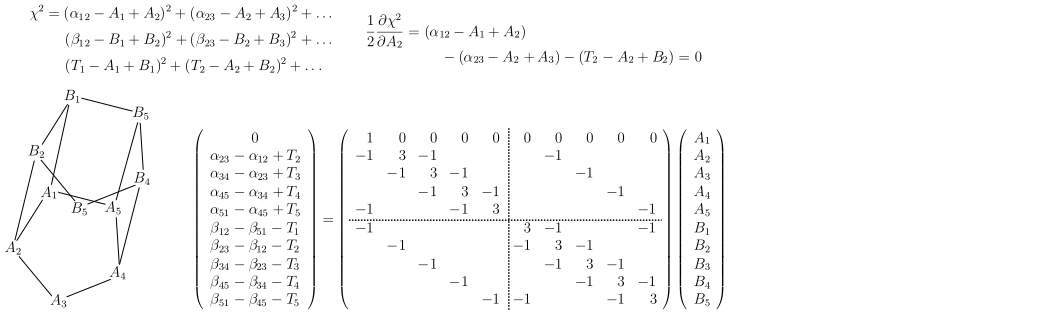
\includegraphics[width=0.9\linewidth]{matrix_description.png}

\vspace{0.2 cm}
\includegraphics[height=0.7\linewidth, angle=90]{final_match.pdf}
\end{center}
\end{frame}

\begin{frame}
\frametitle{Combined fit as seen in overlaps}
\small

\begin{itemize}
\item 

\end{itemize}

\includegraphics[height=\linewidth, angle=90]{final_checkresids_half.pdf}

\end{frame}


%% 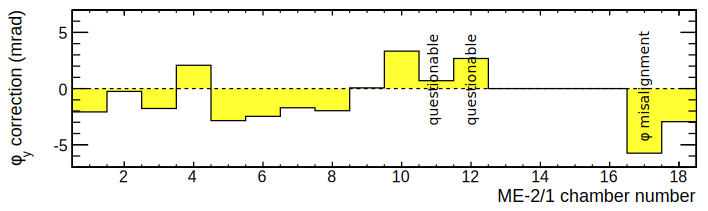
\includegraphics[width=\linewidth]{present21_phiy.pdf}
%% 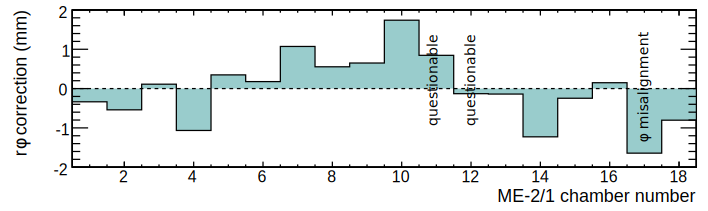
\includegraphics[width=\linewidth]{present21_rphi.pdf}
%% 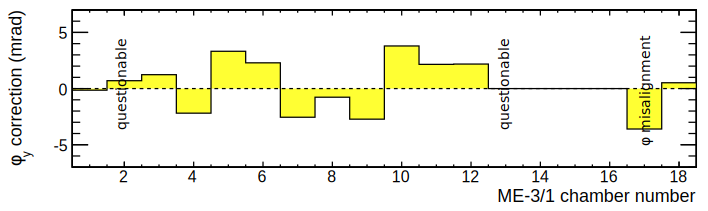
\includegraphics[width=\linewidth]{present31_phiy.pdf}
%% 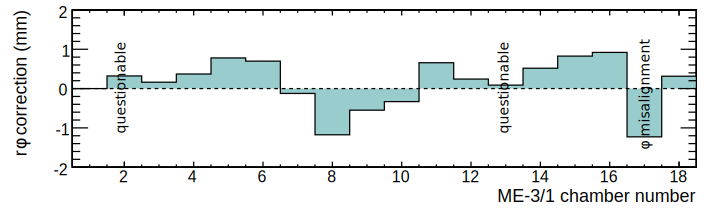
\includegraphics[width=\linewidth]{present31_rphi.pdf}



\begin{frame}
\label{numpages}
\end{frame}

\end{document}
